%!TEX root = practicum2.tex
\Cref{alg:percolation} presents our iterative growth process, the method \FuncSty{percolation} expects three arguments \t{N}, \t{probability} and \t{mask}. Given the size parameter \t{N}, the grid used for the percolation is $(2N + 1) \times (2N + 1)$, since this causes the grid to have an uneven number of rows and columns. The grids center is now always clearly defined as $(N + 1, N + 1)$. The parameter $p \in [0, 1]$ is the probability that a given site in the cluster becomes occupied. The \t{mask} is a binary matrix with $r$ rows and $c$ columns that determines the used connectivity. Until \cref{ss:exp:connectivity} we only consider four-connected clusters for which the mask presented in \cref{fig:exp:connectivity:fourMask} is used.\\

\begin{figure*}
	\centering	
	\begin{subfigure}{0.27\textwidth}
		\centering
		
\includegraphics[width=0.9\textwidth]{./img/fancy_cluster_N20_p3_rng_8}
		\caption{$N = 20$ and $p = 0.3$}
		\label{fig:method:fin_inf:finiteSmall}
	\end{subfigure}
	\begin{subfigure}{0.27\textwidth}
		\centering
		
\includegraphics[width=0.9\textwidth]{./img/fancy_cluster_N20_p5_rng_8}
		\caption{$N = 20$ and $p = 0.5$}
		\label{fig:method:fin_inf:finiteLarge}
	\end{subfigure}	
	\begin{subfigure}{0.27\textwidth}
		\centering
		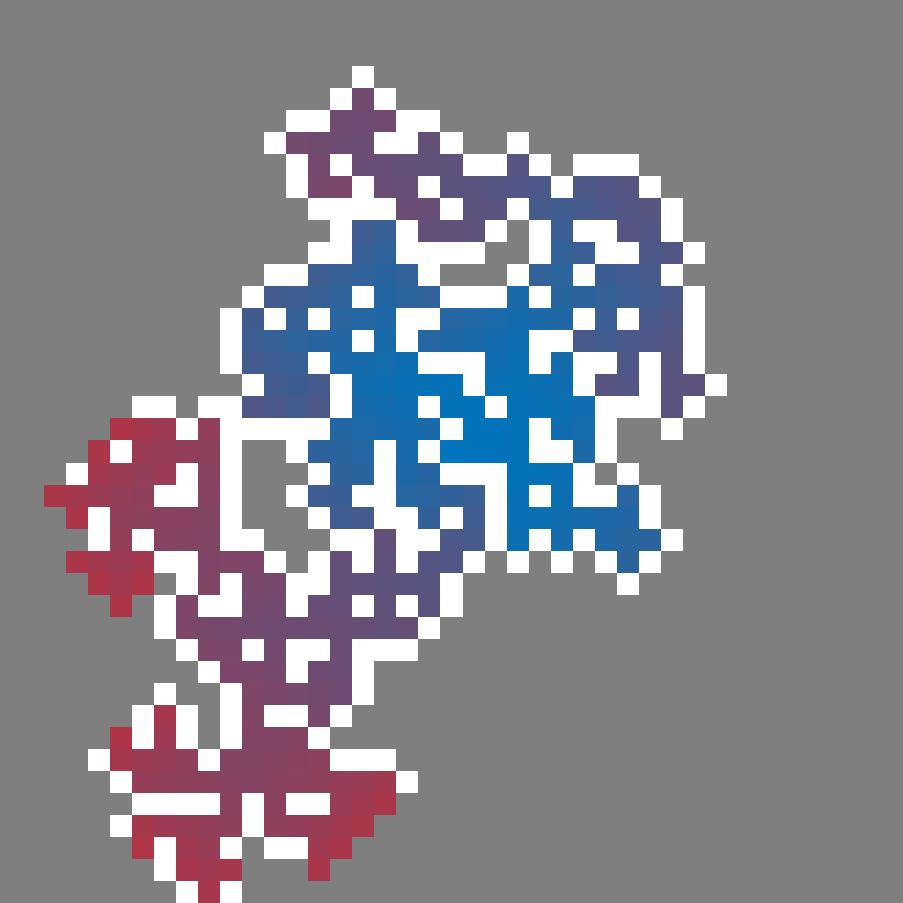
\includegraphics[width=0.9\textwidth]{./img/fancy_cluster_N20_p6_rng_5}
		\caption{$N = 20$ and $p = 0.6$}
		\label{fig:method:fin_inf:infinite}
	\end{subfigure}		
	\caption{Examples of \subref{fig:method:fin_inf:finiteSmall} a small finite cluster, \subref{fig:method:fin_inf:finiteLarge} a larger finite cluster and \subref{fig:method:fin_inf:infinite} a percolating cluster using four-connected neighbours. The colours of the elements in the cluster indicate when that point was added to the cluster, the `colder' the color the earlier in the percolation it was added to the cluster. White cells are empty and gray cells are undetermined. }
	\label{fig:method:fin_inf}
\end{figure*}

\begin{algorithm}[t]
	\setstretch{1.2}
	\SetAlgoShortEnd
	\DontPrintSemicolon
	\SetKwInOut{Input}{input}\SetKwInOut{Output}{output}
	\Input{$N$ size\\
		$p$ probability\\
		$mask$ $r \times c$ binary matrix.}
	\Output{$grid$ $(2N + 1) \times (2N + 1)$ matrix}
	\BlankLine

	$center$ := ($N + 1$, $N + 1$)\; 
	\FuncSty{push($queue$, $center$)}\; 
	$grid$ := \FuncSty{initGrid($N$, $N$)}\; 

	\While{not \FuncSty{isEmpty($queue$)}}{
		$site$ = \FuncSty{pop($queue$)}\; 
		$sites$ = \FuncSty{grow}($grid$, $site$, $mask$, $p$)\; 
		\If{anyOnBorder(sites)}{
			\KwSty{break}
		} 
		\FuncSty{push($queue$, $sites$)}\; 
	}\; 
	\caption{\FuncSty{percolation}$(mask, N, p)$\label{alg:percolation}}
\end{algorithm}

% Initialisation
Initially the only site we have to consider is the center site, which is consequently the only site in the queue at the first iteration.

% Iteratie
Each iteration we pop the next \t{site} from the queue. We grow this point, using the function \t{grow}. This method considers all neighbors that are connected to \t{site} determined by the discussed \t{mask}. For each of these neighbors we generate the value $z$, which is randomly sampled from an uniform distribution with the range $[0,1]$. If $z \leq p$ we mark the neighbor site as occupied, otherwise it is marked empty. The method \t{grow} returns the newly occupied neighboring sites, which are then added to the queue, so they can be processed by the \t{grow} process in a later iteration.

% Stop conditions
The growth of the clusters stops when the queue is empty and it thus cannot grow anymore or if it has reached one of the borders of the grid. In the first case the cluster is finite, which means that all neighboring sites of the cluster, according to the connectivity defined by the \t{mask}, are marked as empty. In \cref{alg:percolation} we test for this condition via the guard of the loop; if the queue is empty there are no more neighbors to consider, consequently the cluster must be finite. 

A percolating cluster is a cluster that has reached the border of the grid, i.e. if there is an occupied site with row or column number $1$ or $2N + 1$. We test for this condition with the method \t{onBorder}. It should be noted that we stop the growth process as soon as a site, that is on the border, enters the queue.\\
% Which has a consequence...

\Cref{fig:method:fin_inf} presents three clusters grown with \cref{alg:percolation}. We can clearly see that the finite clusters are completely surrounded by a white border, which indicates that these sites are empty and processed. \Cref{fig:method:fin_inf:infinite} shows a percolating cluster, which has stopped growing due to a site in the lower left corner.
\todo[inline]{Anders formuleren!!}
Another indication of the percolating nature of the cluster is the fact that there are occupied sites that can still grow, as indicated by their empty neighbours.

